% Options for packages loaded elsewhere
\PassOptionsToPackage{unicode}{hyperref}
\PassOptionsToPackage{hyphens}{url}
\PassOptionsToPackage{dvipsnames,svgnames,x11names}{xcolor}
%
\documentclass[
]{article}

\usepackage{amsmath,amssymb}
\usepackage{setspace}
\usepackage{iftex}
\ifPDFTeX
  \usepackage[T1]{fontenc}
  \usepackage[utf8]{inputenc}
  \usepackage{textcomp} % provide euro and other symbols
\else % if luatex or xetex
  \usepackage{unicode-math}
  \defaultfontfeatures{Scale=MatchLowercase}
  \defaultfontfeatures[\rmfamily]{Ligatures=TeX,Scale=1}
\fi
\usepackage{lmodern}
\ifPDFTeX\else  
    % xetex/luatex font selection
  \setmainfont[]{Nimbus Sans}
  \setmonofont[]{DejaVu Sans Mono}
\fi
% Use upquote if available, for straight quotes in verbatim environments
\IfFileExists{upquote.sty}{\usepackage{upquote}}{}
\IfFileExists{microtype.sty}{% use microtype if available
  \usepackage[]{microtype}
  \UseMicrotypeSet[protrusion]{basicmath} % disable protrusion for tt fonts
}{}
\makeatletter
\@ifundefined{KOMAClassName}{% if non-KOMA class
  \IfFileExists{parskip.sty}{%
    \usepackage{parskip}
  }{% else
    \setlength{\parindent}{0pt}
    \setlength{\parskip}{6pt plus 2pt minus 1pt}}
}{% if KOMA class
  \KOMAoptions{parskip=half}}
\makeatother
\usepackage{xcolor}
\usepackage[margin=1.0in]{geometry}
\setlength{\emergencystretch}{3em} % prevent overfull lines
\setcounter{secnumdepth}{-\maxdimen} % remove section numbering
% Make \paragraph and \subparagraph free-standing
\ifx\paragraph\undefined\else
  \let\oldparagraph\paragraph
  \renewcommand{\paragraph}[1]{\oldparagraph{#1}\mbox{}}
\fi
\ifx\subparagraph\undefined\else
  \let\oldsubparagraph\subparagraph
  \renewcommand{\subparagraph}[1]{\oldsubparagraph{#1}\mbox{}}
\fi

\usepackage{color}
\usepackage{fancyvrb}
\newcommand{\VerbBar}{|}
\newcommand{\VERB}{\Verb[commandchars=\\\{\}]}
\DefineVerbatimEnvironment{Highlighting}{Verbatim}{commandchars=\\\{\}}
% Add ',fontsize=\small' for more characters per line
\newenvironment{Shaded}{}{}
\newcommand{\AlertTok}[1]{\textcolor[rgb]{0.58,0.85,0.30}{\textbf{\colorbox[rgb]{0.30,0.12,0.14}{#1}}}}
\newcommand{\AnnotationTok}[1]{\textcolor[rgb]{0.31,0.63,0.31}{#1}}
\newcommand{\AttributeTok}[1]{\textcolor[rgb]{0.65,0.15,0.64}{#1}}
\newcommand{\BaseNTok}[1]{\textcolor[rgb]{0.60,0.41,0.00}{#1}}
\newcommand{\BuiltInTok}[1]{\textcolor[rgb]{0.65,0.15,0.64}{#1}}
\newcommand{\CharTok}[1]{\textcolor[rgb]{0.31,0.63,0.31}{#1}}
\newcommand{\CommentTok}[1]{\textcolor[rgb]{0.63,0.63,0.65}{\textit{#1}}}
\newcommand{\CommentVarTok}[1]{\textcolor[rgb]{0.89,0.34,0.29}{\textit{#1}}}
\newcommand{\ConstantTok}[1]{\textcolor[rgb]{0.60,0.41,0.00}{#1}}
\newcommand{\ControlFlowTok}[1]{\textcolor[rgb]{0.65,0.15,0.64}{#1}}
\newcommand{\DataTypeTok}[1]{\textcolor[rgb]{0.65,0.15,0.64}{#1}}
\newcommand{\DecValTok}[1]{\textcolor[rgb]{0.60,0.41,0.00}{#1}}
\newcommand{\DocumentationTok}[1]{\textcolor[rgb]{0.89,0.34,0.29}{#1}}
\newcommand{\ErrorTok}[1]{\textcolor[rgb]{0.96,0.28,0.28}{\underline{#1}}}
\newcommand{\ExtensionTok}[1]{\textcolor[rgb]{0.25,0.47,0.95}{\textbf{#1}}}
\newcommand{\FloatTok}[1]{\textcolor[rgb]{0.60,0.41,0.00}{#1}}
\newcommand{\FunctionTok}[1]{\textcolor[rgb]{0.25,0.47,0.95}{#1}}
\newcommand{\ImportTok}[1]{\textcolor[rgb]{0.31,0.63,0.31}{#1}}
\newcommand{\InformationTok}[1]{\textcolor[rgb]{0.77,0.36,0.00}{#1}}
\newcommand{\KeywordTok}[1]{\textcolor[rgb]{0.65,0.15,0.64}{#1}}
\newcommand{\NormalTok}[1]{\textcolor[rgb]{0.22,0.23,0.26}{#1}}
\newcommand{\OperatorTok}[1]{\textcolor[rgb]{0.65,0.15,0.64}{#1}}
\newcommand{\OtherTok}[1]{\textcolor[rgb]{0.15,0.68,0.38}{#1}}
\newcommand{\PreprocessorTok}[1]{\textcolor[rgb]{0.65,0.15,0.64}{#1}}
\newcommand{\RegionMarkerTok}[1]{\textcolor[rgb]{0.16,0.50,0.73}{\colorbox[rgb]{0.08,0.19,0.26}{#1}}}
\newcommand{\SpecialCharTok}[1]{\textcolor[rgb]{0.00,0.52,0.74}{#1}}
\newcommand{\SpecialStringTok}[1]{\textcolor[rgb]{0.85,0.27,0.33}{#1}}
\newcommand{\StringTok}[1]{\textcolor[rgb]{0.31,0.63,0.31}{#1}}
\newcommand{\VariableTok}[1]{\textcolor[rgb]{0.89,0.34,0.29}{#1}}
\newcommand{\VerbatimStringTok}[1]{\textcolor[rgb]{0.85,0.27,0.33}{#1}}
\newcommand{\WarningTok}[1]{\textcolor[rgb]{0.85,0.27,0.33}{#1}}

\providecommand{\tightlist}{%
  \setlength{\itemsep}{0pt}\setlength{\parskip}{0pt}}\usepackage{longtable,booktabs,array}
\usepackage{calc} % for calculating minipage widths
% Correct order of tables after \paragraph or \subparagraph
\usepackage{etoolbox}
\makeatletter
\patchcmd\longtable{\par}{\if@noskipsec\mbox{}\fi\par}{}{}
\makeatother
% Allow footnotes in longtable head/foot
\IfFileExists{footnotehyper.sty}{\usepackage{footnotehyper}}{\usepackage{footnote}}
\makesavenoteenv{longtable}
\usepackage{graphicx}
\makeatletter
\def\maxwidth{\ifdim\Gin@nat@width>\linewidth\linewidth\else\Gin@nat@width\fi}
\def\maxheight{\ifdim\Gin@nat@height>\textheight\textheight\else\Gin@nat@height\fi}
\makeatother
% Scale images if necessary, so that they will not overflow the page
% margins by default, and it is still possible to overwrite the defaults
% using explicit options in \includegraphics[width, height, ...]{}
\setkeys{Gin}{width=\maxwidth,height=\maxheight,keepaspectratio}
% Set default figure placement to htbp
\makeatletter
\def\fps@figure{htbp}
\makeatother

\makeatletter
\@ifpackageloaded{caption}{}{\usepackage{caption}}
\AtBeginDocument{%
\ifdefined\contentsname
  \renewcommand*\contentsname{Table of contents}
\else
  \newcommand\contentsname{Table of contents}
\fi
\ifdefined\listfigurename
  \renewcommand*\listfigurename{List of Figures}
\else
  \newcommand\listfigurename{List of Figures}
\fi
\ifdefined\listtablename
  \renewcommand*\listtablename{List of Tables}
\else
  \newcommand\listtablename{List of Tables}
\fi
\ifdefined\figurename
  \renewcommand*\figurename{Figure}
\else
  \newcommand\figurename{Figure}
\fi
\ifdefined\tablename
  \renewcommand*\tablename{Table}
\else
  \newcommand\tablename{Table}
\fi
}
\@ifpackageloaded{float}{}{\usepackage{float}}
\floatstyle{ruled}
\@ifundefined{c@chapter}{\newfloat{codelisting}{h}{lop}}{\newfloat{codelisting}{h}{lop}[chapter]}
\floatname{codelisting}{Listing}
\newcommand*\listoflistings{\listof{codelisting}{List of Listings}}
\makeatother
\makeatletter
\makeatother
\makeatletter
\@ifpackageloaded{caption}{}{\usepackage{caption}}
\@ifpackageloaded{subcaption}{}{\usepackage{subcaption}}
\makeatother
\makeatletter
\@ifpackageloaded{tcolorbox}{}{\usepackage[skins,breakable]{tcolorbox}}
\makeatother
\makeatletter
\@ifundefined{shadecolor}{\definecolor{shadecolor}{HTML}{FFFFFF}}{}
\makeatother
\makeatletter
\@ifundefined{codebgcolor}{\definecolor{codebgcolor}{HTML}{F3F3F3}}{}
\makeatother
\makeatletter
\ifdefined\Shaded\renewenvironment{Shaded}{\begin{tcolorbox}[sharp corners, frame hidden, borderline west={3pt}{0pt}{shadecolor}, colback={codebgcolor}, enhanced, breakable, boxrule=0pt]}{\end{tcolorbox}}\fi
\makeatother
\ifLuaTeX
  \usepackage{selnolig}  % disable illegal ligatures
\fi
\usepackage{bookmark}

\IfFileExists{xurl.sty}{\usepackage{xurl}}{} % add URL line breaks if available
\urlstyle{same} % disable monospaced font for URLs
\hypersetup{
  colorlinks=true,
  linkcolor={blue},
  filecolor={Maroon},
  citecolor={Blue},
  urlcolor={Blue},
  pdfcreator={LaTeX via pandoc}}

\author{}
\date{}

\begin{document}

\renewcommand*\contentsname{Supplemental text: Review of code used by
Martino et al.}
{
\hypersetup{linkcolor=}
\setcounter{tocdepth}{3}
\tableofcontents
}
\setstretch{1.75}
\raggedright

The code chunks displayed below are copied directly from the code used
by Martino and the line numbers correspond to the indicated files. The
hyperlinks in the text go to the GitHub repository for the
\href{https://github.com/SchlossLab/Schloss_RPCA_XXXXXX_2024}{current
project}, which is a copy of the
\href{https://github.com/cameronmartino/deicode-benchmarking}{original
repository} developed by Martino. Martino's repository was
\href{https://github.com/biocore/DEICODE/commit/ea7835b9a0d16c35685542a81d05ee12c412c6ba}{forked
from the Deicode repository} January 28, 2019. The only changes between
the Martino repository and the copy for this project was to make the
directory and file names lowercase and to replace hyphens with
underscores.

\section{Review of code used to generate positive and negative control
heatmaps in Figure 3DE of
Martino}\label{review-of-code-used-to-generate-positive-and-negative-control-heatmaps-in-figure-3de-of-martino}

Review of the code in
\href{https://github.com/SchlossLab/Schloss_RPCA_XXXXXX_2024/blob/main/deicode_benchmarking/simulations/negative_control.ipynb}{\texttt{deicode\_benchmarking/simulations/negative\_control.ipynb}}
reveals two important problems with the generation of Figure 3DE from
Martino. For background, the \texttt{X\_random} and \texttt{X\_signal}
matrices represented the negative and positive controls, respectively,
that were generated in an earlier block of this notebook. For both
matrices, there were 1000 rows for each feature or taxon and 200 columns
for each sample. At L13 and L15 of block 183, the
\href{https://matplotlib.org/stable/api/_as_gen/matplotlib.pyplot.imshow.html}{\texttt{imshow}
function} from the pyplot package within the \texttt{matplotlib} Python
library is used to generate heatmaps of the two matrices.

\setstretch{1.0}\footnotesize

\begin{Shaded}
\begin{Highlighting}[numbers=left,,firstnumber=10,]
\CommentTok{\#show the results}
\NormalTok{fig,((ax1,ax2),(ax3,ax4)) }\OperatorTok{=}\NormalTok{ plt.subplots(}\DecValTok{2}\NormalTok{,}\DecValTok{2}\NormalTok{,figsize}\OperatorTok{=}\NormalTok{(}\DecValTok{12}\NormalTok{,}\DecValTok{8}\NormalTok{))}

\NormalTok{ax1.imshow(clr(X\_signal}\OperatorTok{+}\DecValTok{1}\NormalTok{),aspect}\OperatorTok{=}\StringTok{\textquotesingle{}auto\textquotesingle{}}\NormalTok{,norm}\OperatorTok{=}\NormalTok{MidpointNormalize(midpoint}\OperatorTok{=}\FloatTok{0.}\NormalTok{), cmap}\OperatorTok{=}\StringTok{\textquotesingle{}PiYG\textquotesingle{}}\NormalTok{)}
\NormalTok{ax1.set\_title(}\StringTok{\textquotesingle{}Positive Control Simulation\textquotesingle{}}\NormalTok{,fontsize}\OperatorTok{=}\DecValTok{22}\NormalTok{)}
\NormalTok{cbim }\OperatorTok{=}\NormalTok{ ax2.imshow(clr(X\_random}\OperatorTok{+}\DecValTok{1}\NormalTok{),aspect}\OperatorTok{=}\StringTok{\textquotesingle{}auto\textquotesingle{}}\NormalTok{,norm}\OperatorTok{=}\NormalTok{MidpointNormalize(midpoint}\OperatorTok{=}\FloatTok{0.}\NormalTok{), cmap}\OperatorTok{=}\StringTok{\textquotesingle{}PiYG\textquotesingle{}}\NormalTok{)}
\NormalTok{ax2.set\_title(}\StringTok{\textquotesingle{}Negative Control Simulation\textquotesingle{}}\NormalTok{,fontsize}\OperatorTok{=}\DecValTok{22}\NormalTok{)}
\end{Highlighting}
\end{Shaded}

\normalsize\setstretch{1.75}

Within the arguments to \texttt{imshow}, the matrices are transformed by
adding 1 to each cell and then subjecting the matrices to a central log
ratio transformation with the
\href{https://scikit.bio/docs/dev/generated/skbio.stats.composition.clr.html\#skbio.stats.composition.clr}{\texttt{clr}
function} from the composition statistics module of the \texttt{skbio}
Python library. It is important to note that the \texttt{clr} function
assumes that the rows represent compositions or samples and the columns
represent the components or taxa. Therefore, \texttt{X\_random} and
\texttt{X\_signal} should have been transposed prior to performing the
clr transformation. For example, on L2 and L6, the matrices were
transposed prior to using the \texttt{rclr} function.

\setstretch{1.0}\footnotesize

\begin{Shaded}
\begin{Highlighting}[numbers=left,,firstnumber=2,]
\CommentTok{\#RPCA on random}
\NormalTok{X\_random\_rclr }\OperatorTok{=}\NormalTok{ rclr().fit\_transform(X\_random.T)}
\NormalTok{opt\_noise }\OperatorTok{=}\NormalTok{ OptSpace().fit(X\_random\_rclr)}
\NormalTok{U\_random }\OperatorTok{=}\NormalTok{ pd.DataFrame(opt\_noise.sample\_weights,index}\OperatorTok{=}\NormalTok{X\_random.columns)}
\CommentTok{\#RPCA on very clear signal}
\NormalTok{X\_signal\_rclr }\OperatorTok{=}\NormalTok{ rclr().fit\_transform(X\_signal.T)}
\NormalTok{opt\_sig }\OperatorTok{=}\NormalTok{ OptSpace().fit(X\_signal\_rclr)}
\NormalTok{U\_signal }\OperatorTok{=}\NormalTok{ pd.DataFrame(opt\_sig.sample\_weights,index}\OperatorTok{=}\NormalTok{X\_signal.columns)}
\end{Highlighting}
\end{Shaded}

\normalsize\setstretch{1.75}

As executed in the notebook, the result of using the \texttt{clr}
function was the same shape as the input matrices with features as rows
and samples as columns. The transformed data were then used in the
\texttt{imshow} function which plots the rows and columns of the matrix
to the rows and columns of the heatmap. However, at L21-24 ``Samples''
is added to the y-axis label and ``Features'' is added to the x-axis
label, which is the reverse of the actual situation. These problems in
visually representing the simulated data hid the fact that samples
rather than taxa were shared between the treatment groups.

\setstretch{1.0}\footnotesize

\begin{Shaded}
\begin{Highlighting}[numbers=left,,firstnumber=21,]
\NormalTok{ax2.set\_ylabel(}\StringTok{\textquotesingle{}Samples\textquotesingle{}}\NormalTok{,fontsize}\OperatorTok{=}\DecValTok{15}\NormalTok{)}
\NormalTok{ax1.set\_ylabel(}\StringTok{\textquotesingle{}Samples\textquotesingle{}}\NormalTok{,fontsize}\OperatorTok{=}\DecValTok{15}\NormalTok{)}
\NormalTok{ax2.set\_xlabel(}\StringTok{\textquotesingle{}Features\textquotesingle{}}\NormalTok{,fontsize}\OperatorTok{=}\DecValTok{15}\NormalTok{)}
\NormalTok{ax1.set\_xlabel(}\StringTok{\textquotesingle{}Features\textquotesingle{}}\NormalTok{,fontsize}\OperatorTok{=}\DecValTok{15}\NormalTok{)}
\end{Highlighting}
\end{Shaded}

\normalsize\setstretch{1.75}

The problem with the labelling of the axes can more clearly be seen by
changing the value of the \texttt{aspect} argument in \texttt{imshow}
from \texttt{\textquotesingle{}auto\textquotesingle{}} to \texttt{None}
on L13-14. To summarize, the code in this block (i) performed the CLR
transformation across the samples rather than across the taxa and (ii)
mislabelled the axes of the heatmaps in Figure 3DE of Martino. Both
problems could have been avoided by transposing the matrices within the
arguments to \texttt{clr} at L13 and L15. The result is shown below on
the right.

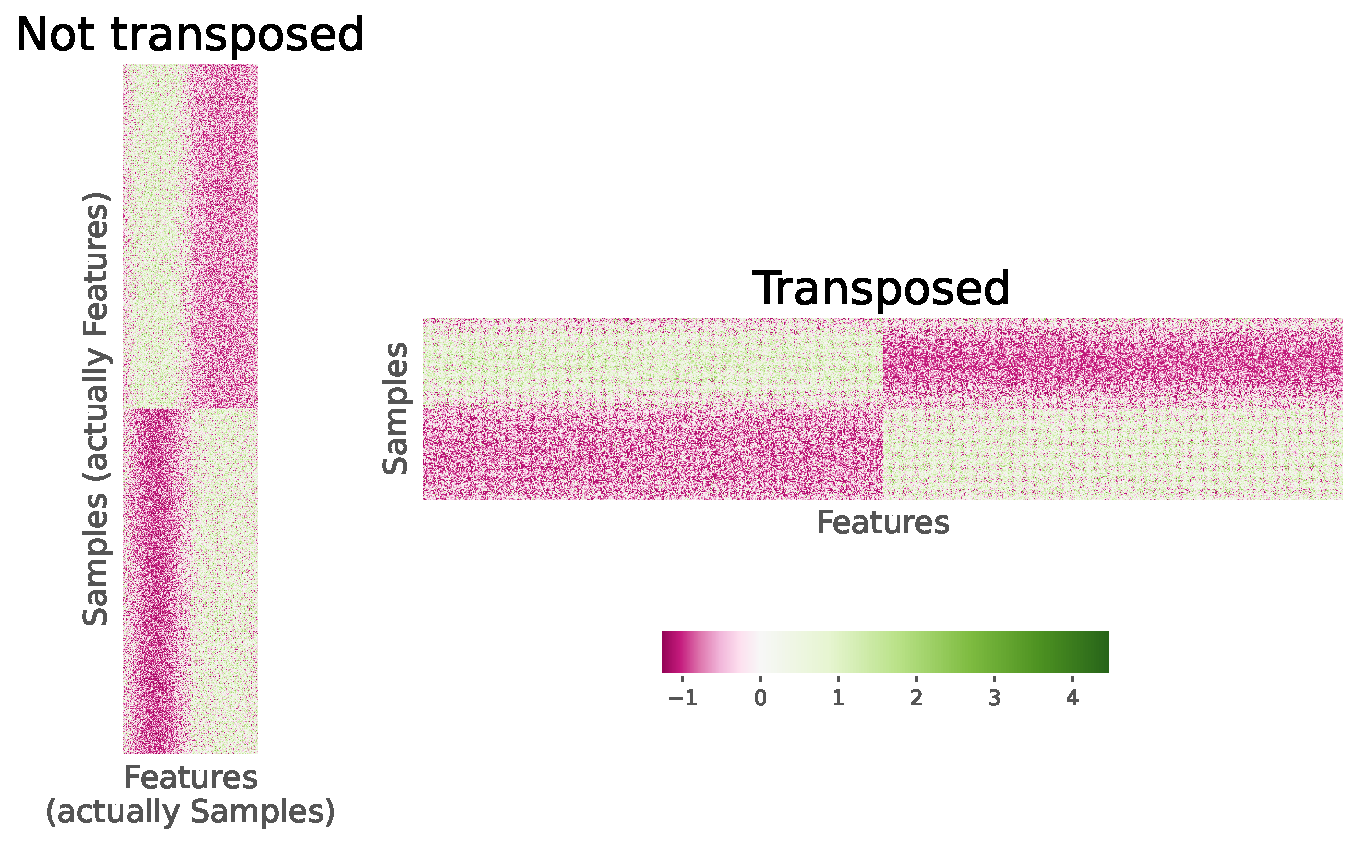
\includegraphics{supplemental_text_files/figure-pdf/cell-4-output-1.pdf}

\section{\texorpdfstring{Review of \texttt{build\_block\_model} function
and its
dependencies}{Review of build\_block\_model function and its dependencies}}\label{review-of-build_block_model-function-and-its-dependencies}

The
\href{https://github.com/SchlossLab/Schloss_RPCA_XXXXXX_2024/blob/main/deicode_benchmarking/simulations/scripts/simulations.py\#L175}{\texttt{build\_block\_model}}
and related functions can be found in
\href{https://github.com/SchlossLab/Schloss_RPCA_XXXXXX_2024/blob/main/deicode_benchmarking/simulations/scripts/simulations.py}{\texttt{deicode\_benchmarking/simulations/scripts/simulations.py}}.
The function is called in
\texttt{deicode\_benchmarking/simulations/negative\_control.ipynb} to
generate the positive control data in Figure 3D and in
\texttt{deicode\_benchmarking/simulations/scripts/cluster\_build.py} to
generate the overlapping data analyzed in Figure 3ABC of Martino. The
\texttt{build\_block\_model} function is listed below except for lines
corresponding to comments (L185-236) and code that did not impact the
generation of \texttt{X\_noise} (L244-253 and L262-267). The function
returned the values of \texttt{X\_true} and \texttt{X\_noise}.

\setstretch{1.0}\footnotesize

\begin{Shaded}
\begin{Highlighting}[numbers=left,,firstnumber=175,]
\KeywordTok{def}\NormalTok{ build\_block\_model(}
\NormalTok{        rank,}
\NormalTok{        hoced,}
\NormalTok{        hsced,}
\NormalTok{        spar,}
\NormalTok{        C\_,}
\NormalTok{        num\_samples,}
\NormalTok{        num\_features,}
\NormalTok{        overlap}\OperatorTok{=}\DecValTok{0}\NormalTok{,}
\NormalTok{        mapping\_on}\OperatorTok{=}\VariableTok{True}\NormalTok{):}
\end{Highlighting}
\end{Shaded}

\normalsize\setstretch{1.75}

\setstretch{1.0}\footnotesize

\begin{Shaded}
\begin{Highlighting}[numbers=left,,firstnumber=237,]
\NormalTok{    X\_true }\OperatorTok{=}\NormalTok{ block\_diagonal\_gaus(}
\NormalTok{      num\_samples,}
\NormalTok{      num\_features,}
\NormalTok{      rank,}
\NormalTok{      overlap,}
\NormalTok{      minval}\OperatorTok{=}\FloatTok{.01}\NormalTok{,}
\NormalTok{      maxval}\OperatorTok{=}\NormalTok{C\_)}
\end{Highlighting}
\end{Shaded}

\normalsize\setstretch{1.75}

\setstretch{1.0}\footnotesize

\begin{Shaded}
\begin{Highlighting}[numbers=left,,firstnumber=254,]
\NormalTok{    X\_noise }\OperatorTok{=}\NormalTok{ X\_true.copy()}
\NormalTok{    X\_noise }\OperatorTok{=}\NormalTok{ np.array(X\_noise)}
    \CommentTok{\# add Homoscedastic noise}
\NormalTok{    X\_noise }\OperatorTok{=}\NormalTok{ Homoscedastic(X\_noise, hoced)}
    \CommentTok{\# add Heteroscedastic noise}
\NormalTok{    X\_noise }\OperatorTok{=}\NormalTok{ Heteroscedastic(X\_noise, hsced)}
    \CommentTok{\# Induce low{-}density into the matrix}
\NormalTok{    X\_noise }\OperatorTok{=}\NormalTok{ Subsample(X\_noise, spar, num\_samples)}
\end{Highlighting}
\end{Shaded}

\normalsize\setstretch{1.75}

As called in \texttt{cluster\_build.py}, the value of \texttt{rank} was
2 corresponding to the number of treatment groups, \texttt{num\_samples}
was 200, \texttt{num\_features} was 1000, and \texttt{overlap} was 20
(\texttt{overlap} was zero in the positive control analysis). The values
of \texttt{hoced}, \texttt{hsced}, \texttt{spar}, and \texttt{C\_} were
based on a parameter that was altered for each sequencing depth. For
example, to generate samples with 4000 sequences, the parameter of 2500
was used. The \texttt{spar} and \texttt{C\_} values were set to the
parameter value (e.g., 2500) and were used to scale the relative
abundance values in the \texttt{Subsample} (L261) and
\texttt{block\_diagonal\_gaus} (L237-243) functions, respectively. As
used in the overlap analysis, the \texttt{hoced} and \texttt{hsced}
values were set to the parameter value divided by 15; for the positive
control analysis they were divided by 60. These values were used in the
\texttt{Homoscedastic} (L257) and \texttt{Heteroscedastic} (L259)
functions where \texttt{hoced} and \texttt{hsced} were used to set the
standard deviation of a normal distribution with mean set to the
relative abundance of the sample-taxon pair receiving additional noise
uniformly or randomly. The parameter values used in
\texttt{build\_block\_model} were selected by fitting the model to
experimental data from a study comparing the microbial communities on
subject's fingers and keyboards. Although I did not attempt to replicate
their model fitting, other code is found in \texttt{simulations.py} that
ostensibly performs this analysis.

A general problem with the code in \texttt{simulations.py} was that if I
loaded \texttt{simulations.py} and ran \texttt{build\_block\_model}
multiple times with the same input data and random number generator
seed, the code did not produce the same results. Although not a critical
problem, the lack of computational reproducibility was part of the
motivation to assess the benchmarking test results with ten seeds.

Finally, one of the comments describes \texttt{build\_block\_model} as
returning a data frame with \texttt{num\_samples} rows and
\texttt{num\_features} columns.

\setstretch{1.0}\footnotesize

\begin{Shaded}
\begin{Highlighting}[numbers=left,,firstnumber=223,]
\NormalTok{    Returns}
    \OperatorTok{{-}{-}{-}{-}{-}{-}{-}}
\NormalTok{    Pandas Dataframes}
\NormalTok{    Table }\ControlFlowTok{with}\NormalTok{ a block diagonal where the rows represent samples}
    \KeywordTok{and}\NormalTok{ the columns represent features.  The values within the blocks}
\NormalTok{    are gaussian.}
\end{Highlighting}
\end{Shaded}

\normalsize\setstretch{1.75}

In fact, it returns a data frame with \texttt{num\_features} rows and
\texttt{num\_samples} columns. This confusion might help explain why
samples rather than features overlap in the
\texttt{block\_diagonal\_gaus} function as written. This issue is
described in the next section.

\subsection{\texorpdfstring{Review of \texttt{block\_diagonal\_gaus}
function}{Review of block\_diagonal\_gaus function}}\label{review-of-block_diagonal_gaus-function}

The function
\href{https://github.com/SchlossLab/Schloss_RPCA_XXXXXX_2024/blob/main/deicode_benchmarking/simulations/scripts/simulations.py\#73}{\texttt{block\_diagonal\_gaus}}
is called by \texttt{build\_block\_model} and is also found in
\href{https://github.com/SchlossLab/Schloss_RPCA_XXXXXX_2024/blob/main/deicode_benchmarking/simulations/scripts/simulations.py}{\texttt{deicode\_benchmarking/simulations/scripts/simulations.py}}.

\setstretch{1.0}\footnotesize

\begin{Shaded}
\begin{Highlighting}[numbers=left,,firstnumber=73,]
\KeywordTok{def}\NormalTok{ block\_diagonal\_gaus(}
\NormalTok{        ncols,}
\NormalTok{        nrows,}
\NormalTok{        nblocks,}
\NormalTok{        overlap}\OperatorTok{=}\DecValTok{0}\NormalTok{,}
\NormalTok{        minval}\OperatorTok{=}\DecValTok{0}\NormalTok{,}
\NormalTok{        maxval}\OperatorTok{=}\FloatTok{1.0}\NormalTok{):}
\end{Highlighting}
\end{Shaded}

\normalsize\setstretch{1.75}

As used in Martino, \texttt{ncols} was 200 and \texttt{nrows} was 1000.
As described in the Methods of the original study, the model uses a
normal distribution to vary the relative abundance of each taxa with
different distributions for each treatment group such that a specified
fraction of taxa overlapped between the two treatment groups. Within
\texttt{block\_diagonal\_gaus} the number of treatment groups was
specified with \texttt{nblocks}, which was 2 and the overlap was
specified with \texttt{overlap}, which was 20 for the overlapping
conditions and 0 for the positive control. The value of \texttt{maxval}
was used to scale relative abundance values in the function and was set
to the parameter described in the previous section (e.g., 2500 for a
sequence depth of 4000). The function generates a matrix with
\texttt{ncols} samples and \texttt{nrows} taxa; however, comments in the
function describe a transposed version of the matrix.

\setstretch{1.0}\footnotesize

\begin{Shaded}
\begin{Highlighting}[numbers=left,,firstnumber=105,]
\NormalTok{    Returns}
    \OperatorTok{{-}{-}{-}{-}{-}{-}{-}}
\NormalTok{    np.array}
\NormalTok{        Table }\ControlFlowTok{with}\NormalTok{ a block diagonal where the rows represent samples}
        \KeywordTok{and}\NormalTok{ the columns represent features.  The values within the blocks}
\NormalTok{        are gaussian distributed between }\DecValTok{0} \KeywordTok{and} \FloatTok{1.}
\end{Highlighting}
\end{Shaded}

\normalsize\setstretch{1.75}

In addition, as I'll show below, the output is not a block diagonal.

The function begins by initializing a matrix with zeroes and a graidient
of values to define a distribution.

\setstretch{1.0}\footnotesize

\begin{Shaded}
\begin{Highlighting}[numbers=left,,firstnumber=117,]
    \ControlFlowTok{if}\NormalTok{ nblocks }\OperatorTok{\textless{}=} \DecValTok{1}\NormalTok{:}
        \ControlFlowTok{raise} \PreprocessorTok{ValueError}\NormalTok{(}\StringTok{\textquotesingle{}\textasciigrave{}nblocks\textasciigrave{} needs to be greater than 1.\textquotesingle{}}\NormalTok{)}
\NormalTok{    mat }\OperatorTok{=}\NormalTok{ np.zeros((nrows, ncols))}
\NormalTok{    gradient }\OperatorTok{=}\NormalTok{ np.linspace(}\DecValTok{0}\NormalTok{, }\DecValTok{10}\NormalTok{, nrows)}
\NormalTok{    mu }\OperatorTok{=}\NormalTok{ np.linspace(}\DecValTok{0}\NormalTok{, }\DecValTok{10}\NormalTok{, ncols)}
\NormalTok{    sigma }\OperatorTok{=} \DecValTok{1}
\NormalTok{    xs }\OperatorTok{=}\NormalTok{ [norm.pdf(gradient, loc}\OperatorTok{=}\NormalTok{mu[i], scale}\OperatorTok{=}\NormalTok{sigma)}
          \ControlFlowTok{for}\NormalTok{ i }\KeywordTok{in} \BuiltInTok{range}\NormalTok{(}\BuiltInTok{len}\NormalTok{(mu))]}
\NormalTok{    mat }\OperatorTok{=}\NormalTok{ np.vstack(xs).T}
\end{Highlighting}
\end{Shaded}

\normalsize\setstretch{1.75}

This code is largely superfluous since the values of these values are
written over by subsequent code before the matrix (i.e., \texttt{mat})
is updated. Regardless, operationally, \texttt{mat} is defined as a
matrix of zeroes with \texttt{num\_features} rows and
\texttt{num\_samples} columns (L188). A vector with
\texttt{num\_features} values, \texttt{gradient}, is defined as a linear
interpolation between the values of 0 and 10 (L189). Similarly, a vector
with \texttt{num\_samples} values, \texttt{mu}, is defined as a linear
interpolation between the values of 0 and 10 (L190). These values along
with a \texttt{sigma} value of 1 are used to create a
\texttt{num\_samples} long vector of arrays called, which are each
\texttt{num\_features} long (L123-124). This vector of arrays,
\texttt{xs}, takes its values from the Normal probability density
function at the \texttt{num\_features} values of \texttt{gradient} under
a distribution with a mean at each of the \texttt{num\_samples} values
of \texttt{mu} with a standard deviation of \texttt{sigma} (i.e., 1).
The \texttt{num\_features} by \texttt{num\_samples} matrix \texttt{mat}
is generated by combining each element of \texttt{xs} as the columns. As
suggested in the comment above from L171, this matrix has maximum
probabilities along the diagonal of the matrix. Values far off the
diagonal are nearly zero. For example, the value for the first feature
in the first sample was 0.3989 and it was 7.7e-23 in the last sample.
The following is a heatmap visualization of the raw values in the matrix
(the matrix has been transposed).

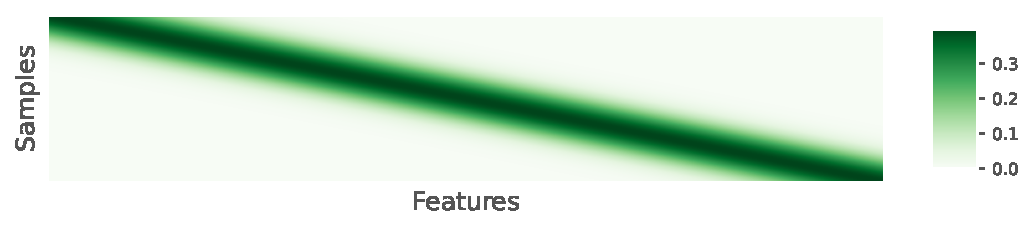
\includegraphics{supplemental_text_files/figure-pdf/cell-6-output-1.pdf}

As stated in the description of L117-125, the values of \texttt{mat} are
largely overwritten by the following lines of code.

\setstretch{1.0}\footnotesize

\begin{Shaded}
\begin{Highlighting}[numbers=left,,firstnumber=127,]
\NormalTok{    block\_cols }\OperatorTok{=}\NormalTok{ ncols }\OperatorTok{//}\NormalTok{ nblocks}
\NormalTok{    block\_rows }\OperatorTok{=}\NormalTok{ nrows }\OperatorTok{//}\NormalTok{ nblocks}
    \ControlFlowTok{for}\NormalTok{ b }\KeywordTok{in} \BuiltInTok{range}\NormalTok{(nblocks }\OperatorTok{{-}} \DecValTok{1}\NormalTok{):}

\NormalTok{      gradient }\OperatorTok{=}\NormalTok{ np.linspace(}\DecValTok{5}\NormalTok{, }\DecValTok{5}\NormalTok{, block\_rows)  }\CommentTok{\# samples (bock\_rows)}
      \CommentTok{\# features (block\_cols+overlap)}
\NormalTok{      mu }\OperatorTok{=}\NormalTok{ np.linspace(}\DecValTok{0}\NormalTok{, }\DecValTok{10}\NormalTok{, block\_cols }\OperatorTok{+}\NormalTok{ overlap)}
\NormalTok{      sigma }\OperatorTok{=} \FloatTok{2.0}
\NormalTok{      xs }\OperatorTok{=}\NormalTok{ [norm.pdf(gradient, loc}\OperatorTok{=}\NormalTok{mu[i], scale}\OperatorTok{=}\NormalTok{sigma)}
            \ControlFlowTok{for}\NormalTok{ i }\KeywordTok{in} \BuiltInTok{range}\NormalTok{(}\BuiltInTok{len}\NormalTok{(mu))]}

\NormalTok{      B }\OperatorTok{=}\NormalTok{ np.vstack(xs).T }\OperatorTok{*}\NormalTok{ maxval}
\NormalTok{              lower\_row }\OperatorTok{=}\NormalTok{ block\_rows }\OperatorTok{*}\NormalTok{ b}
\NormalTok{              upper\_row }\OperatorTok{=} \BuiltInTok{min}\NormalTok{(block\_rows }\OperatorTok{*}\NormalTok{ (b }\OperatorTok{+} \DecValTok{1}\NormalTok{), nrows)}
\NormalTok{              lower\_col }\OperatorTok{=}\NormalTok{ block\_cols }\OperatorTok{*}\NormalTok{ b}
\NormalTok{              upper\_col }\OperatorTok{=} \BuiltInTok{min}\NormalTok{(block\_cols }\OperatorTok{*}\NormalTok{ (b }\OperatorTok{+} \DecValTok{1}\NormalTok{), ncols)}

              \ControlFlowTok{if}\NormalTok{ b }\OperatorTok{==} \DecValTok{0}\NormalTok{:}
\NormalTok{                  mat[lower\_row:upper\_row, lower\_col:}\BuiltInTok{int}\NormalTok{(upper\_col }\OperatorTok{+}\NormalTok{ overlap)] }\OperatorTok{=}\NormalTok{ B}
              \ControlFlowTok{else}\NormalTok{:}
\NormalTok{                  ov\_tmp }\OperatorTok{=} \BuiltInTok{int}\NormalTok{(overlap }\OperatorTok{/} \DecValTok{2}\NormalTok{)}
                  \ControlFlowTok{if}\NormalTok{ (B.shape) }\OperatorTok{==}\NormalTok{ (mat[lower\_row:upper\_row,}
\end{Highlighting}
\end{Shaded}

\normalsize\setstretch{1.75}

L127 and L128 define the number of columns (\texttt{block\_cols}) and
rows (\texttt{block\_rows}) in each block. Because \texttt{nblocks} is 2
for all simulations, these values become 100 and 500, respectively. At
L129, a loop is initiated for values of the index variable \texttt{b},
which ranges between 0 and the integer less than \texttt{nblocks-1} or
0. Therefore, the loop is only executed once and the else statement at
L146-159 is never executed. At L131 and L133 new versions of
\texttt{gradient} and \texttt{mu} are generated. The values in
\texttt{gradient} are all 5 and the values in \texttt{mu} are taken from
a linear extrapolation between 0 and 10. Here is evidence for the
overlap of samples rather than features. The vector \texttt{mu} has
\texttt{block\_cols} (i.e., 100) plus \texttt{overlap} (i.e., 20)
values. Because the columns contain sample data the additional 20
columns represent 20 additional samples rather than features. The code
that was described at L123-125 is repeated as L135-138, using a standard
deviation of 2 rather than 1. The resulting matrix, \texttt{B}, has 500
rows and 120 columns. Each row of \texttt{B} is identical with the
columns being the value of the probability distribution function at 5.0
(i.e., \texttt{gradient} as defined at L131) for a normal distribution
with the 120 values of \texttt{mu} as the mean and 2.0 (i.e.,
\texttt{sigma}) as the standard deviation. At L145, this matrix is used
to replace the values in the upper left quadrant of \texttt{mat} in
L139-145. The values of the first 500 rows in the last 80 columns are
all nearly zero and are taken from the value of \texttt{mat} generated
at L125.

\setstretch{1.0}\footnotesize

\begin{Shaded}
\begin{Highlighting}[numbers=left,,firstnumber=161,]
\NormalTok{    upper\_col }\OperatorTok{=} \BuiltInTok{int}\NormalTok{(upper\_col }\OperatorTok{{-}}\NormalTok{ overlap)}
    \CommentTok{\# Make last block fill in the remainder}
\NormalTok{    gradient }\OperatorTok{=}\NormalTok{ np.linspace(}\DecValTok{5}\NormalTok{, }\DecValTok{5}\NormalTok{, nrows }\OperatorTok{{-}}\NormalTok{ upper\_row)}
\NormalTok{    mu }\OperatorTok{=}\NormalTok{ np.linspace(}\DecValTok{0}\NormalTok{, }\DecValTok{10}\NormalTok{, ncols }\OperatorTok{{-}}\NormalTok{ upper\_col)}
\NormalTok{    sigma }\OperatorTok{=} \DecValTok{4}
\NormalTok{    xs }\OperatorTok{=}\NormalTok{ [norm.pdf(gradient, loc}\OperatorTok{=}\NormalTok{mu[i], scale}\OperatorTok{=}\NormalTok{sigma)}
          \ControlFlowTok{for}\NormalTok{ i }\KeywordTok{in} \BuiltInTok{range}\NormalTok{(}\BuiltInTok{len}\NormalTok{(mu))]}
\NormalTok{    B }\OperatorTok{=}\NormalTok{ np.vstack(xs).T }\OperatorTok{*}\NormalTok{ maxval}

\NormalTok{    mat[upper\_row:, upper\_col:] }\OperatorTok{=}\NormalTok{ B}
\end{Highlighting}
\end{Shaded}

\normalsize\setstretch{1.75}

The code shown here is very similar to what was done at L131-138. The
only difference was that in this chunk they used a standard deviation of
4.0 (i.e., \texttt{sigma}) instead of 2.0. The new value of \texttt{B}
defined at L168 was used to complete the value of \texttt{mat} by
filling in the last 500 rows and the last 120 columns (L170). Again, the
values of the first 80 columns in the last 500 rows were nearly zero.

In conclusion there were three issues with the code in the
\texttt{block\_diagonal\_gaus} function. First, the code at the
beginning of the function (L117-125) was extraneous. Second, and more
important, the features had the same relative abundance within each
sample. Finally, and perhaps most important, samples were shared across
features rather than features being shared across samples. As written in
the original Jupyter notebook, the at the end of the
\texttt{block\_diagonal\_gaus} function, using values of \texttt{ncols}
set to 200, \texttt{nrows} to 1000, \texttt{nblocks} to 2,
\texttt{overlap} to 20, and \texttt{maxval} to 2500 resulted in a 1000
row by 200 column matrix. This is a heatmap depiction of the raw values
in \texttt{mat} with lighter colors are lower abundance while darker
colors are higher abundance.

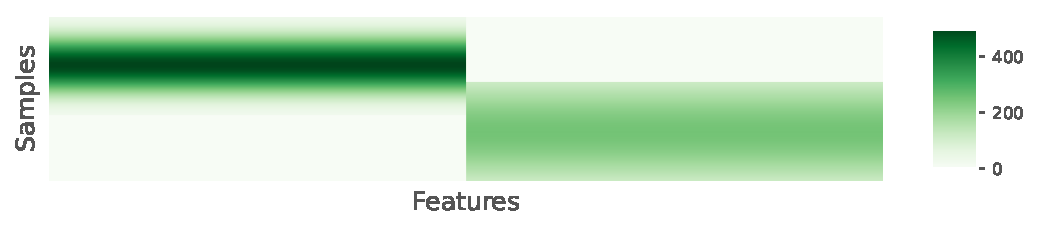
\includegraphics{supplemental_text_files/figure-pdf/cell-7-output-1.pdf}

To highlight the observation that the probabilities were the same for
each feature across non-overlapping samples within the same block, the
following heatmap shows the relative abundances of each feature:

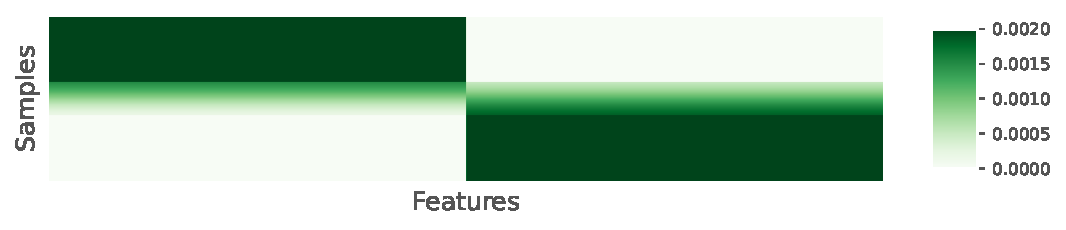
\includegraphics{supplemental_text_files/figure-pdf/cell-8-output-1.pdf}

\subsection{\texorpdfstring{Review of
\texttt{Homoscedastic}}{Review of Homoscedastic}}\label{review-of-homoscedastic}

The \texttt{Homoscedastic} function applies noise randomly sampled from
a normal distribution to each sample-taxon pair of the matrix using the
abundance of the sample-taxon pair as the mean and \texttt{intensity} as
the standard deviation. For the cases where overlap was included between
the treatment groups, the intensity was the model parameter (e.g., 2500)
divided by 15 (i.e., 166.6667) and for the case where there was no
overlap between the treatment groups, the intensity was the model
parameter divided by 60 (i.e., 41.6667).

\setstretch{1.0}\footnotesize

\begin{Shaded}
\begin{Highlighting}[numbers=left,,firstnumber=42,]
\KeywordTok{def}\NormalTok{ Homoscedastic(X\_noise, intensity):}
    \CommentTok{""" uniform normally dist. noise """}
\NormalTok{    X\_noise }\OperatorTok{=}\NormalTok{ np.array(X\_noise)}
\NormalTok{    err }\OperatorTok{=}\NormalTok{ intensity }\OperatorTok{*}\NormalTok{ np.ones\_like(X\_noise.copy())}
\NormalTok{    X\_noise }\OperatorTok{=}\NormalTok{ rand.normal(X\_noise.copy(), err)}

    \ControlFlowTok{return}\NormalTok{ X\_noise}
\end{Highlighting}
\end{Shaded}

\normalsize\setstretch{1.75}

The code from L42-48 shows a potential problem. The median abundance in
\texttt{X\_noise} coming into \texttt{Homoscedastic} across all samples
was 115.7 with a maximum value of 498.6. Considering that random numbers
were drawn from distributions with a standard deviation of 166.67 it was
likely that negative values would result. In fact, for this example,
28.5\% of the sample-taxon pairs were negative. It is likely that the
normal distribution should have been truncated by turning negative
values to zeroes. Below is a heatmap depiction of \texttt{X\_noise}
after L257 of the \texttt{build\_block\_model} function in
\texttt{simulations.py}.

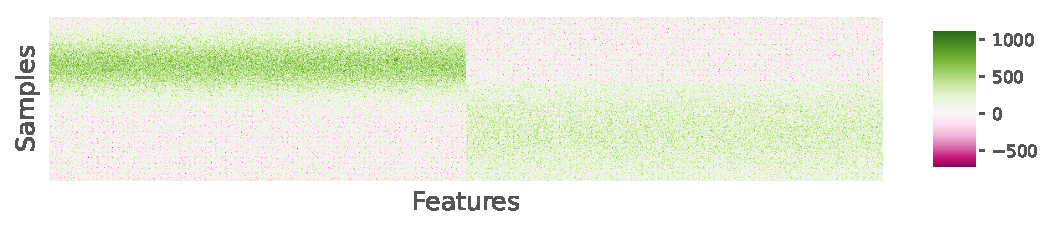
\includegraphics{supplemental_text_files/figure-pdf/cell-10-output-1.pdf}

\subsection{\texorpdfstring{Review of
\texttt{Heteroscedastic}}{Review of Heteroscedastic}}\label{review-of-heteroscedastic}

Similar to \texttt{Homoscedastic}, the \texttt{Heteroscedastic} function
applies noise randomly sampled from a normal distribution using the
abundance of the sample-taxon pair from \texttt{X\_noise} as the mean
and \texttt{intensity} as the standard deviation. Again, for the cases
where overlap was included between the treatment groups, the intensity
was the model parameter (e.g., 2500) divided by 15 (i.e., 166.6667) and
for the case where there was no overlap between the treatment groups,
the intensity was the model parameter divided by 60 (i.e., 41.6667). The
primary difference from \texttt{Homoscedastic} is that
\texttt{Heteroscedastic} only applies the noise to a random subset of
the sample-taxon pairs. Although this was how the second of three
sources of noise was described in the ``Simulations'' subsection of the
``Materials and Methods'' section of Martino, review of the code shows
that it applied the noise to all values of \texttt{X\_noise} rather than
to a subset.

\setstretch{1.0}\footnotesize

\begin{Shaded}
\begin{Highlighting}[numbers=left,,firstnumber=51,]
\KeywordTok{def}\NormalTok{ Heteroscedastic(X\_noise, intensity):}
    \CommentTok{""" non{-}uniform normally dist. noise """}
\NormalTok{    err }\OperatorTok{=}\NormalTok{ intensity }\OperatorTok{*}\NormalTok{ np.ones\_like(X\_noise)}
\NormalTok{    i }\OperatorTok{=}\NormalTok{ rand.randint(}\DecValTok{0}\NormalTok{, err.shape[}\DecValTok{0}\NormalTok{], }\DecValTok{5000}\NormalTok{)}
\NormalTok{    j }\OperatorTok{=}\NormalTok{ rand.randint(}\DecValTok{0}\NormalTok{, err.shape[}\DecValTok{1}\NormalTok{], }\DecValTok{5000}\NormalTok{)}
\NormalTok{    err[i, j] }\OperatorTok{=}\NormalTok{ intensity}
\NormalTok{    X\_noise }\OperatorTok{=} \BuiltInTok{abs}\NormalTok{(rand.normal(X\_noise, err))}

    \ControlFlowTok{return}\NormalTok{ X\_noise}
\end{Highlighting}
\end{Shaded}

\normalsize\setstretch{1.75}

At L53 the code generates \texttt{err}, which is a matrix with the same
dimensions as \texttt{X\_noise} where every cell has the value of the
intensity (e.g.,166.67). On L53-54 they select 5000 random row and
column indices that are then used in L55 to assign values of
\texttt{err} to \texttt{intensity}. L53-55 do not change the existing
values of \texttt{err} since the values in the matrix were all already
set to the value of \texttt{intensity} at L494. At L498 noise is added
to all values of \texttt{X\_noise} much like was done in
\texttt{Homoscedastic} at L46. It is likely that the authors intended to
use the numpy \texttt{zeros\_like} function on L53 instead of the
\texttt{ones\_like} function. Then at L497, \texttt{err} would have had
5000 cells with the value of \texttt{intensity} and the
\texttt{rand.normal} function would have changed only those values at
L498. One notable difference to \texttt{Homoscedastic} is that L498 uses
\texttt{abs} to return the absolute value of \texttt{rand.normal}. Prior
to applying the absolute value to the abundances with the additional
noise 32.2\% of the sample-taxon pairs were negative. Using \texttt{abs}
would certainly add noise to a subset of \texttt{X\_noise}, but it would
not be random since it would disproportionately impact low abundance
features. As mentioned for \texttt{Homoscedastic} returning zero rather
than negative values or their absolute value would likely have been
preferred. Below is a heatmap depiction of \texttt{X\_noise} after L259
of the \texttt{build\_block\_model} function in \texttt{simulations.py}.

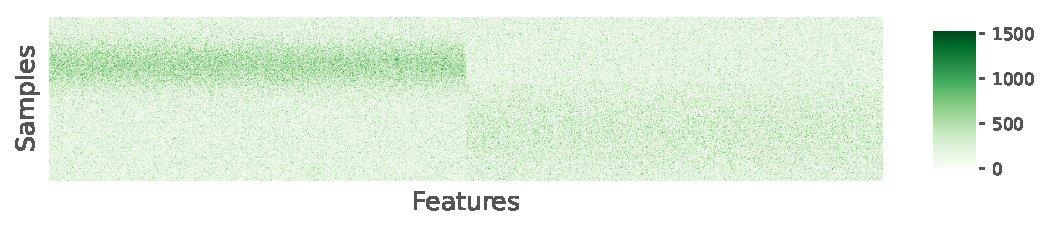
\includegraphics{supplemental_text_files/figure-pdf/cell-12-output-1.pdf}

\subsection{\texorpdfstring{Review of
\texttt{Subsample}}{Review of Subsample}}\label{review-of-subsample}

In the final step of \texttt{simulations.py} the values of
\texttt{X\_noise} are used to generate a count matrix with the desired
number of individuals per sample (L261) using the \texttt{Subsample}
function.

\setstretch{1.0}\footnotesize

\begin{Shaded}
\begin{Highlighting}[numbers=left,,firstnumber=51,]
\KeywordTok{def}\NormalTok{ Subsample(X\_noise, spar, num\_samples):}
    \CommentTok{""" yij \textasciitilde{} PLN( lambda\_\{ij\}, /phi ) """}
    \CommentTok{\# subsample}
\NormalTok{    mu }\OperatorTok{=}\NormalTok{ spar }\OperatorTok{*}\NormalTok{ closure(X\_noise.T).T}
\NormalTok{    X\_noise }\OperatorTok{=}\NormalTok{ np.vstack([poisson(lognormal(np.log(mu[:, i]), }\DecValTok{1}\NormalTok{))}
                         \ControlFlowTok{for}\NormalTok{ i }\KeywordTok{in} \BuiltInTok{range}\NormalTok{(num\_samples)]).T}
    \CommentTok{\# add sparsity}

    \ControlFlowTok{return}\NormalTok{ X\_noise}
\end{Highlighting}
\end{Shaded}

\normalsize\setstretch{1.75}

This function takes \texttt{X\_noise} as input along with the
\texttt{spar} and \texttt{num\_samples} parameters. The value of
\texttt{spar} is the same model parameter value that was used to scale
the relative abundances in \texttt{block\_diagonal\_gaus} (e.g., 2500).
At L531, the relative abundance of features within each sample was
determined and then multiplied by \texttt{spar} to generate \texttt{mu}
which was a \texttt{num\_features} by \texttt{num\_samples} array. These
values were used to generate counts for each sample-taxon pair using a
Poisson-lognormal distribution, which produces a new version of
\texttt{X\_noise}, which was returned to \texttt{build\_block\_model}
and used for the rest of the analysis.

Below is a heatmap depiction of the central log ratio transformation of
\texttt{X\_noise} after adding 1 to each cell at the end of the
\texttt{build\_block\_model} function in \texttt{simulations.py}.

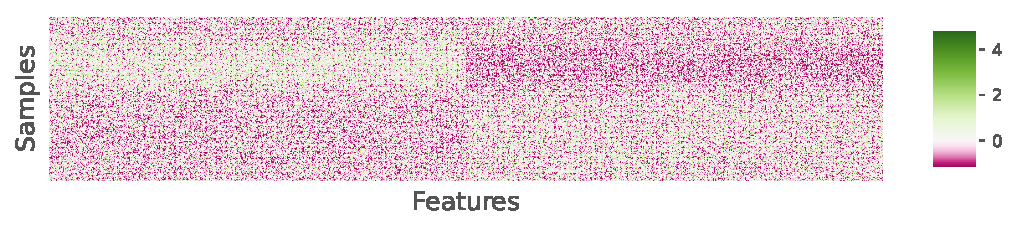
\includegraphics{supplemental_text_files/figure-pdf/cell-14-output-1.pdf}

The matrix generated from \texttt{Subsample} did not have a consistent
total number of counts for each sample. When using the model parameter
of 2500, values near 4000 individuals per sample were obtained, but
there was considerable variation. For the example that has been used in
this review, the mean number of individuals per sample was 4132.9 with a
range between 3628 and 4808. Considering the claim that RPCA is
invariant to differences in sampling effort, it would be desirable to
control whether samples had the same number of individuals. As a
workaround for this problem, I increased the model parameter (e.g.,
2800) so that the minimum sample size was greater than the desired
number of individuals and then down sampled each sample to the desired
number.

\subsection{Summary}\label{summary}

Five problems were found in the code as written in the original
\texttt{simulations.py} script. They are listed here in order of
importance.

\textbf{1. Samples were shared between the two treatment groups.} The
intention was that features should be shared between treatment groups.\\
\textbf{2. Among samples from the same treatment group, the abundance
distributions for each feature were the same.} The result was that the
relative abundance for all features in the same sample and treatment
group had the same expected relative abundance. The intention was likely
that the abundance distribution within each sample varied by feature.\\
\textbf{3. The total number of individuals varied across each sample.}
Although there were claims that RPCA was insensitive to uneven sampling
effort, this was not actually demonstrated in Martino. It was necessary
to make the sampling effort uniform.\\
\textbf{4. The heteroscedastic source of noise was actually applied
noise to all samples.} The result was a second addition of noise to all
sample-taxon values rather than the intended subset of values.\\
\textbf{5. Negative mean values were used as the mean in normal
distribution sampling functions when calculating the heteroscedastic
noise.} It is likely that the intention was for negative values to be
transformed to zeros before sampling the distribution.\\
\textbf{6. The signs of negative values generated after applying the
heteroscedastic noise were made positive.} It is likely that the
intention was for negative values to be transformed to zeros.\\
\textbf{7. Setting the random number generator seed was inadequate to
ensure that rerunning \texttt{simulations.py} with the same parameters
yielded the same result.}

I suspect that the confusion over the information contained in the rows
and columns of the positive and negative controls described above is
related to the first two problems I identified. Taken together, these
problems do not undercut the claims made by Martino about the
performance of RPCA.

Because my analysis expanded upon the benchmarking performed by Martino
to include smaller effect sizes, the code in \texttt{simulations.py} was
unable to adequately simulate the similarity we observe among samples
within and between treatment groups. Therefore, I rewrote
\texttt{simulations.py} as an R script \texttt{simulations.R} (found in
\texttt{workflow/scripts/}) that resolved the above-mentioned problems.



\end{document}
